% Created 2024-05-31 Fri 15:26
% Intended LaTeX compiler: pdflatex
\documentclass[letterpaper, 11pt]{article}
                      \usepackage{lmodern} % Ensures we have the right font
\usepackage[T1]{fontenc}
\usepackage[utf8]{inputenc}
\usepackage{graphicx}
\usepackage{amsmath, amsthm, amssymb}
\usepackage[table, xcdraw]{xcolor}
\definecolor{bblue}{HTML}{0645AD}
\usepackage[colorlinks]{hyperref}
\hypersetup{colorlinks, linkcolor=blue, urlcolor=bblue}
\usepackage{titling}
\setlength{\droptitle}{-6em}
\setlength{\parindent}{0pt}
\setlength{\parskip}{1em}
\usepackage[stretch=10]{microtype}
\usepackage{hyphenat}
\usepackage{ragged2e}
\usepackage{subfig} % Subfigures (not needed in Org I think)
\usepackage{hyperref} % Links
\usepackage{listings} % Code highlighting
\usepackage[top=1in, bottom=1.25in, left=1.55in, right=1.55in]{geometry}
\renewcommand{\baselinestretch}{1.15}
\usepackage[explicit]{titlesec}
\pretitle{\begin{center}\fontsize{20pt}{20pt}\selectfont}
\posttitle{\par\end{center}}
\preauthor{\begin{center}\vspace{-6bp}\fontsize{14pt}{14pt}\selectfont}
\postauthor{\par\end{center}\vspace{-25bp}}
\predate{\begin{center}\fontsize{12pt}{12pt}\selectfont}
\postdate{\par\end{center}\vspace{0em}}
\titlespacing\section{0pt}{5pt}{5pt} % left margin, space before section header, space after section header
\titlespacing\subsection{0pt}{5pt}{-2pt} % left margin, space before subsection header, space after subsection header
\titlespacing\subsubsection{0pt}{5pt}{-2pt} % left margin, space before subsection header, space after subsection header
\usepackage{enumitem}
\setlist{itemsep=-2pt} % or \setlist{noitemsep} to leave space around whole list
\usepackage{tabularx}
\author{Stefan Harris}
\date{}
\title{Computer Science H446 Coursework Project: Pac-Man Game\\\medskip
\large Candidate Number: 1419 Centre Number: 19268}
\hypersetup{
 pdfauthor={Stefan Harris},
 pdftitle={Computer Science H446 Coursework Project: Pac-Man Game},
 pdfkeywords={},
 pdfsubject={},
 pdfcreator={Emacs 29.3 (Org mode 9.6.24)}, 
 pdflang={English}}
\usepackage{biblatex}
\addbibresource{/home/stefan/documents/programming/pac-man-clone/doc/working/bib/sources.bib}
\begin{document}

\maketitle
\tableofcontents


\section{Introduction}
\label{sec:org01a1196}
This project aims to develop a program serving as a recreation of the 1980 coin-op arcade game Pac-Man, using both the household high-level programming language Python and a 3rd party library to enable game development, Pygame.
The project aims at creating a rather conservative recreation of the original.
The core gameplay loop will be retained as much as possible by researching the original game’s mechanics, namely the mechanics of the ghosts: the algorithms that dictate where they will move, where they will move to and how to react to key game play moments.
Any features outside gameplay will be mostly cosmetic and or serves as a quality-of-life improvement for the player.
\section{Analysis}
\label{sec:org4d54335}
\subsection{Identifying the Problem (An Explanation of Pac-Man)}
\label{sec:orga1e2292}
Pac-Man is a 1980 arcade game developed and published by Bandai Namco in Japan.
And published by Midway Games in North America.
Despite initially receiving lukewarm reception in Japan, the game showed both critical and commercial success outside the nation and the franchise remains one of the highest-grossing video game series of all time.

Development of Pac-man begun in 1979, directed by Toru Iwatani with a nine-man team.
Iwatani noticed that most arcade games of the time appealed more to a masculine audience, with conflict being quite unanimous.
Discontent with this, he aimed to create a game that would appeal to woman as well as men.
A colourful art style and game play loop that would appeal to all ages was the idea.

The core gameplay revolves around Pac-Man and his goal, to eat all the pellets/dots in the maze without being caught by the pursuing ghosts.
Pac-man can turn the tables by tactically eating the large dots known as power pellets.
This will frighten the ghosts, making them vulnerable to Pac-Man eating them for bonus points.
Difficulty increases the more levels the player completes, with the ghosts becoming more aggressive among other subtle changes, like power pellets no longer fully functioning.

To add variance to the gameplay, each ghost has their own unique behaviour to catch Pac-Man, giving the illusion that they are working together and making them seem smarter than they are.
They also alternate between behaviour states during a level, namely chase mode –when they are pursuing Pac-Man, and scatter mode – when they flee to the maze’s corners to give the player a breather.

\begin{figure}[htbp]
\centering
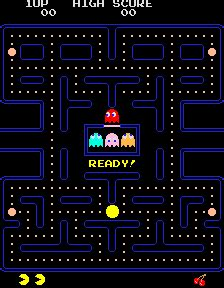
\includegraphics[width=0.5\linewidth]{./img/analysis/pacman-start.jpg}
\caption{\label{fig:pacman-start}The beginning of a game of Pac-Man.}
\end{figure}

\subsection{Solving the Problem using Computational Methods}
\label{sec:org277d725}
\label{Solving the Problem using Computational Methods}
One of the reasons I chose Pac-Man for my coursework is because I believe it serves as a good example on how computational methods can be applied to a large project to make it more approachable.

\subsubsection{Abstraction}
\label{sec:org6767b8f}
Abstraction helps in reducing the amount of hardware resources taken up by the program, ensuring that performance is optimal on the range of target systems.
An abstract model will serve as a representation of reality, only functioning in the ways it needs to.

Pac-Man is already an abstracted form of a chasing simulation.
The game takes place on a 2D plane, yet still provides a good representation of a real-life chase scenario.
The omission of a 3rd dimension results in far less lines of code, storage, and processing, a necessity when acknowledging the limited hardware of the time.
All the entities are sprites consisting of only a couple colours and frames of animation, a drastic simplification of how the characters are depicted in the game’s promotional material and arcade cabinet.
The maze does not represent any real-life location and is represented by simple outlines for walls.
The entities can only move in cardinal directions.

\begin{figure}[htbp]
\centering
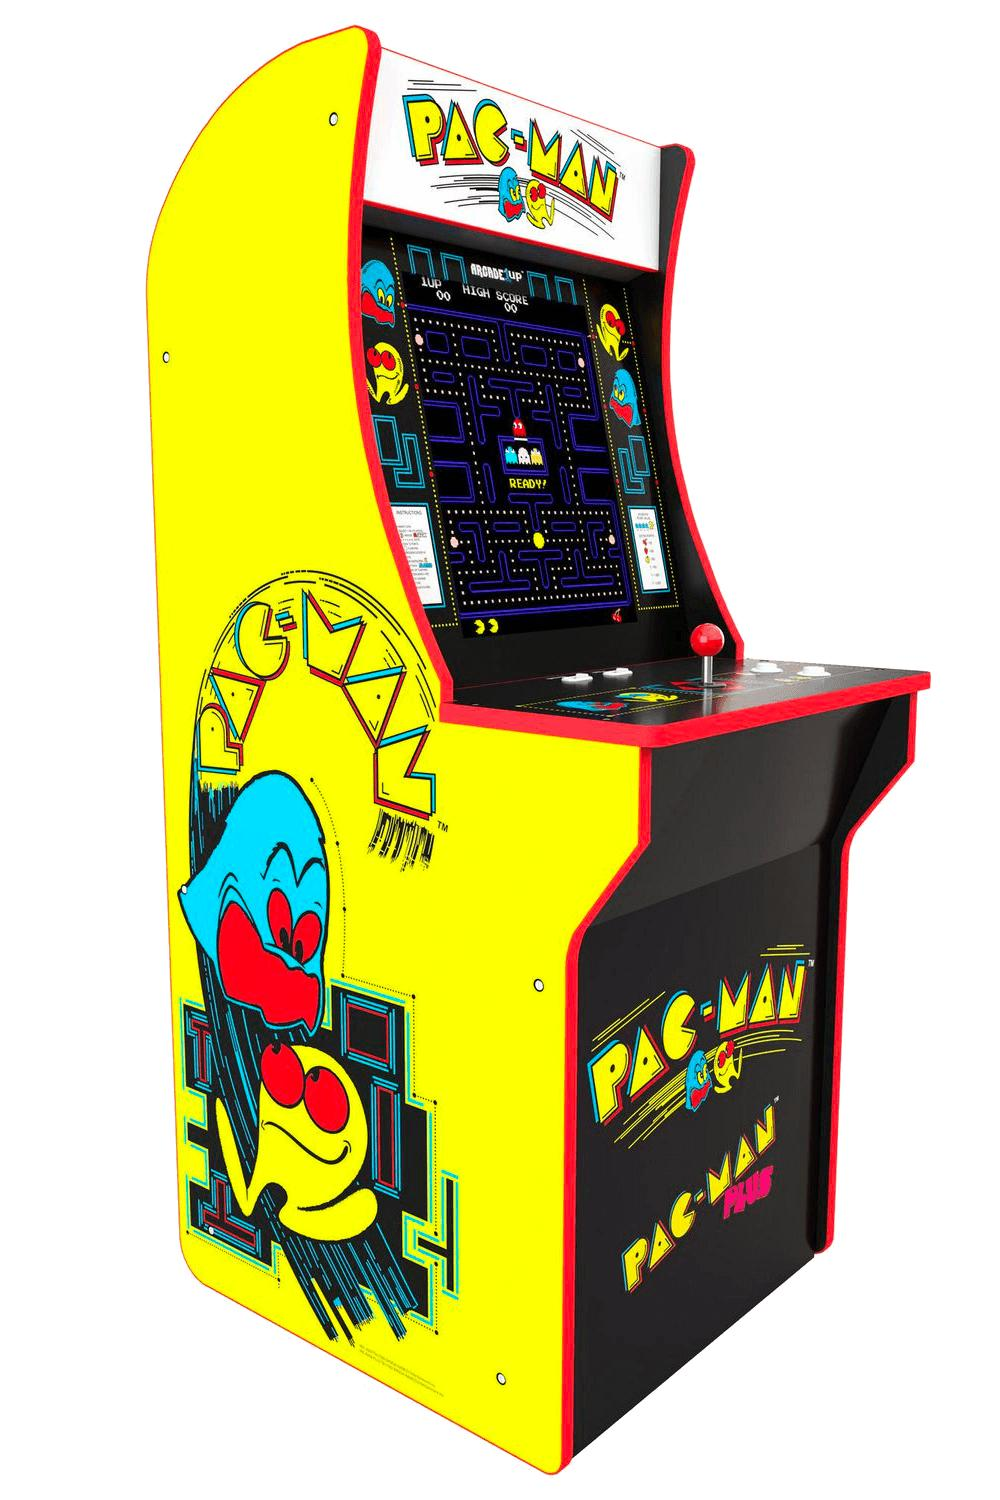
\includegraphics[width=0.33\linewidth]{./img/analysis/arcade-cabinet.jpg}
\caption{\label{fig:arcade-cabinet}An original arcade cabinet. Note how the art on the side doesn't match the game's graphics, but more-so its bright colours.}
\end{figure}

With the source material already being abstracted, it is easy to find and implement the core mechanics into my project such as the player movement, ghost behaviour and ghost states while ignoring more superfluous aspects like cut-scenes between levels.

\subsubsection{Decomposition}
\label{sec:orgd1852d4}
For complex problems like this, decomposition is invaluable for breaking it down into simpler, more manageable chunks that can be prioritised, developed, and tested individually.
It makes life so much easier on the developer’s end.

This solution is no exception, it can be decomposed into its core components.

For example, the core gameplay loop of Pac-Man can be decomposed into a series of entities interacting with each other: Pac-Man, pellets, ghosts, bonus fruit etc.
Each entity can then be further decomposed into their core behaviours.
So, for Pac-man that will be his movement, his eating and dying.
For ghosts, it is their movement algorithm and behaviour states.
Once the game is fully decomposed, the components can then be prioritised, such as the maze being implemented before the gameplay since the maze will house all the gameplay.

\subsubsection{Logic, Branching and Iteration}
\label{sec:orgfccf959}
These are pivotal for adding interactivity and dynamism to the solution.
Without these the code is completely linear and with little to no meaningful interactivity, which is not optimal for a game, a program that is supposed to react to user input.

Iteration is essential because it allows the game to repeat operations indefinitely, significantly reducing the number of lines in the code base.
It also allows the game to run indefinitely via a game loop.

Logic is an integral part of the gameplay; the ghosts will use logical comparisons to decide what will be the next best direction to get themselves closer to Pac-Man or to decide if a direction is eligible to move in or to decide if it is time to switch to a different behaviour state.

Branching in the form of if/else statements must be used for the game to respond to user input and produce an action.
The game can check for user inputs each frame using a series of if statements.
For example, when the player presses the left movement key, Pac-Man will move left, otherwise he will not.

Iteration in the form of for/while loops is integral for the game to run in real-time.
A main game loop will be used to clear the screen, update the entities, and refresh the display for each frame.
Iteration will also be used in entity behaviour; the ghosts will iterate through each cardinal direction to decide what direction to move in.

\subsubsection{Pipelining and Concurrent Thinking}
\label{sec:org1f418df}
Pipelining allows for one process to start while another is finishing.
Concurrency is when multiple processes are split into time slices and ordered into a schedule to be worked on.

These methods allow for an increased program throughput, which is important for a game like this.
The game should run at a consistent frame rate, preferably 60 frames per second; all computation between frames needs to be done within a \textasciitilde{}16.67ms window.
Major drops in framerate will mean choppy movement, stuttering and less responsive controls, the latter being the most unbearable since the game can demand quick reactions.
The throughput pipelining and concurrency offers will ensure that all computation between frames will be done within the window, keeping performance at an optimum.

Concurrent processing via scheduling algorithms is present in almost every modern operating system.
The same can be said for pipelining, which is a mainstay in most contemporary CPU architectures.
These two methods will not need to be explicitly implemented in my code because these are implicit optimizations that are autonomous.

\subsubsection{Performance Modelling}
\label{sec:orgfae8381}
Performance modelling means analysing the performance of algorithms to determine what processes are taking up the most time and addressing them accordingly.
It is vital for the game to run smoothly so that there is minimal delay between the player’s input and what appears on screen.
Excessive frame drops and delayed input can make the game cumbersome to play.
Knowledge of the scalability of algorithms will help in predicting any future performance issues and optimisations.
Big  notation is suitable for this task.
For example, if I know that an algorithm has a time complexity of , I can seek an algorithm that scales better, stopping the poor scalability form becoming an issue later in development.

Python’s built-in libraries such as ‘time’ will be used to measure the elapsed time between an algorithm starting and ending, with this information, it is possible to find the percentage of time an algorithm takes in a single frame or even the approximate number clock cycles it uses.
Optimisations can then be achieved based on this data.
However, knowing the Big O is arguably more beneficial as the time for an algorithm to compute will very across hardware configurations.

\subsubsection{Thinking Ahead}
\label{sec:org730b26f}
This refers to the careful planning to make sure the project is completed to a good standard and within time.
Thinking ahead is useful as it allows you to determine how much time should be spent on each key part of the solution.

I can achieve this by dictating a programming paradigm that the solution will revolve around, which will be Object Oriented Programming (OOP).
By sticking to this, I can plan out how each entity of the game will translate to objects using Unified Modelling Language (UML) diagrams.
OOP lends itself well to reusability and modularity through inheritance and polymorphism.
Which is a big plus for saving time and for keeping the code base clean and simple.

Thinking ahead also refers to caching, the process where frequently accessed data can be temporarily stored somewhere for quick access when needed.
In software this can be a web cache in local storage, in hardware this can be a small primary storage inside a processor.
All modern consumer grade CPUs have a cache that is used implicitly, so I do not need to implement caching in my code.

\subsubsection{Stakeholders}
\label{sec:org8dc0009}
This game can attract a variety of stakeholders, like how the original arcade release aimed to satisfy a wide demographic.
These stakeholders include:

\begin{itemize}
\item \textbf{Children} – Aged 5 to 12, male and female.
Children that have an interest in video games and or play video games as a pastime.
These children may not be very versed in technology but will be able to pick the game up easily due to the simple controls and easy to grasp winning and losing conditions.
They may also be attracted to the colourful appearance of Pac-Man and the ghosts.
The game was designed for an arcade setting, allowing it to be played in short bursts.
Suitable for children with short attention spans.
The score can serve as a gateway to competition amongst a group of children.
While the controls and graphics may be the most important to them, they may ask for a high score/leader board system to further facilitate competition.
While possible, implementing this is not on top of my priority list.
Implementing the gameplay first will not only satisfy all stakeholders, but also guarantees that the game will serve as a strong showcase of \hyperref[Solving the Problem using Computational Methods]{solving a problem using computational methods} and algorithmic thinking within the time that I have.
If I have enough time, I can add these extra features.

\item \textbf{Adults} – Aged 20 to 50, male and female.
 Adults that remember playing the original arcade realise during its peak or remember playing later versions or realises.
 They may be a fan of Pac-Man, looking for a simple way of playing a recreation of Pac-Man without having to toy with emulation or other methods.
 Akin to the children, some adults may not be versed with technology, so they may seek a simple way of playing Pac-Man, which this solution will serve.
 The simple controls and arcade-centric design allows adults to use the game to get some entertainment during their free time.
 While the simplicity of the game can be appealing for young children, it can become boring for adults, they may ask for variety \hyperref[Ms. Pac-Man]{seen in other releases, like multiple maze layouts}.
Again, I want to focus on implementing the core gameplay, with extra features being added if I have enough time.

\item \textbf{Programmers} – Likely hobbyists that have an interest in how retro games work.
These people are likely to have less of an interest in the game and more so on its code.
They may find use in an implementation of Pac-Man’s underlying algorithms in a modern high-level language, they can fork the code for use in their own projects, without having to do research or use an emulator’s disassembler and debugger to try and make sense of the algorithms.
These stakeholders may ask for the source code to be easy to read and understand.
An aspect of my solution that will be a priority.
\end{itemize}

\section{Researching Existing Solutions}
\label{sec:orge36864e}
To replicate the game play of the original Pac-Man, I needed to do some research on existing solutions.
This involved a dive into the original algorithm that dictates how the ghosts traverse the maze, their unique behaviour, and their various states.
With this knowledge I will be able to confidently translate these algorithms into Python and Pygame.

The commercial success of the original of Pac-Man naturally led to many other realises over the years.
Some offer simple quality-of-life improvements, to adding whole new mechanics.
I will assess these features and decide whether to implement them or not.

\subsection{Pac-Man (A Look into Ghost Movement and Behaviour)}
\label{sec:org60cd4d3}
One of the reasons I decided to do this project was because of this comprehensive video I watched a while ago from a YouTube channel called Retro Game Mechanics Explained.
The video goes over every facet of the ghosts’ behaviours in detail.

\begin{figure}[htbp]
\centering
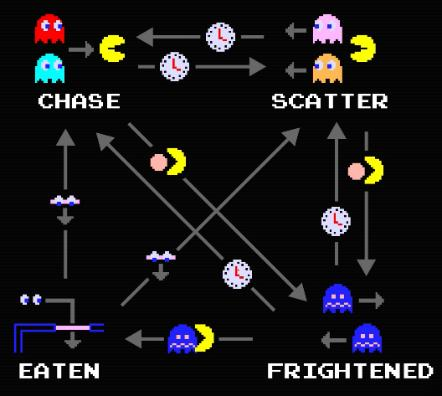
\includegraphics[width=0.33\linewidth]{./img/analysis/retro-game-mech/ghost-states.jpg}
\caption{\label{fig:ghost-states}Video graphic showing the four states and how they interact \autocite{RetroGameMechanicsExplained}.}
\end{figure}

The video begins with an explanation of the four states and how each ghost moves between them.
There are 4 states: chase, scatter, frightened and eaten.
The ghosts will alternate between chase and scatter depending on a timer.
When Pac-Man eats a power pellet, they will temporarily enter frightened mode and then enter eaten mode when Pac-Man touches them.
Upon entering the ghost house, they will regenerate and either enter scatter or chase depending on the timer.
This is something that I will definitely add.

The video then explains the timings for scatter and chase mode, with the quirk of Blinky constantly being in chase mode when there are only a few dots left in the maze, something that I will also add.

An explanation of the movement algorithm is then given.
The ghosts use a targeting system to determine the tile to move towards.
Each cardinal direction is checked to see if it’s a valid direction to move in.
A direction is considered invalid if it leads into a wall or causes them move back the way they came.
Out of the valid directions, the distance between the tile the direction will lead to and the target is calculated.
The direction that yields the smallest number will be the direction the ghost will move in.
If all directions yield the same distance a priority system is used to pick one.
Up is given the highest priority, then left, down and right.
All of this will be included.

\begin{figure}[htbp]
\centering
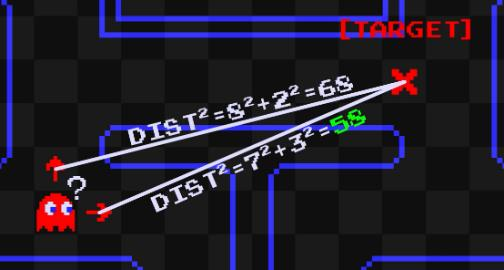
\includegraphics[width=0.50\linewidth]{./img/analysis/retro-game-mech/choose-direction.jpg}
\caption{\label{fig:choose-direction}Video graphic showing Blinky choosing a direction \autocite{RetroGameMechanicsExplained}.}
\end{figure}

The various modes are then explained.
During scatter mode, the ghosts’ target tile is set to a corner of the maze.
When chasing, Blinky’s target tile is directly on Pac-Man, Pinky’s is four tiles ahead, Inky’s is dependant on Blinky’s and Pac-Mans postion, and Clyde is on Pac-Man, until he gets within eight tiles of him, in which case he will scatter away for several seconds.
When frightened the ghosts will u-turn and begin to move in random, eligible directions according to a random number generator (RNG).
All this will be added.

The video addresses a bug that occurs when multiplying the ‘up’ unit vector.
The code that handles applying magnitude to unit vectors treats the x and y components as one 16-bit value rather than two 8-bit ones, leading to the multiplication of the y component overflowing into the x.
For Pinky this means that her target tile is three tiles up and four left when Pac-man is facing upwards.
This is obviously a bug, therefore I won’t replicate it in my solution.

\begin{figure}[htbp]
\centering
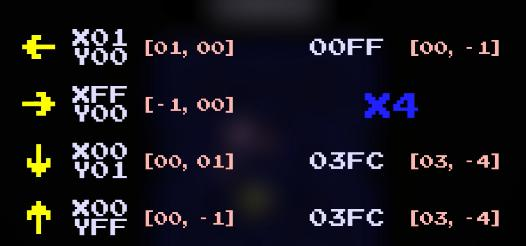
\includegraphics[width=0.50\linewidth]{./img/analysis/retro-game-mech/pinky-bug.jpg}
\caption{\label{fig:pinky-bug}Video Graphic showing the overflow error. Multiplying \texttt{\$FF} by 4 makes \texttt{\$3FC}. The left most nibble overflows into the x component. \autocite{RetroGameMechanicsExplained}.}
\end{figure}

\subsection{Ms. Pac-Man}
\label{sec:org1f6245b}
\label{Ms. Pac-Man}
Released in 1982 by publisher Midway, Ms Pac-Man is the questionably licensed sequel to Namco’s original arcade release.

\begin{figure}[htbp]
\centering
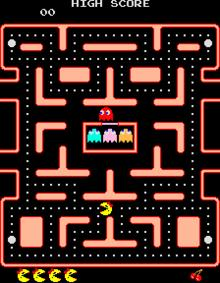
\includegraphics[width=0.33\linewidth]{./img/analysis/ms-pac-man/start.jpg}
\caption{\label{fig:ms-pacman-start}Start of a game of Ms. Pac-Man. Note how the walls are now solid pink and that they’re now two sets of warp tunnels.}
\end{figure}

The gameplay does not stray far away from the original, instead it adds new quality-of-life improvements and new content that still retains the timelessness of the original’s gameplay:

\begin{itemize}
\item The maze walls are now filled with a solid colour that contrasts better with the black rather than being simple outlines that can blend into the background, especially so considering the blur CRT displays have, which were in ubiquitous during the era Pac-Man came out in.
This offers a nice usability feature for the visually impaired, who may struggle to distinguish the walls from the background.
This is something that I will certainly implement into my solution.
\item One gameplay enhancement comes from the ghost behaviour.
At the start of the level, Blinky and Pinky ghosts will move randomly for the first couple of seconds before falling into their typical behaviour.
This not only adds a small ripple to the gameplay for experienced players but can also serve a good challenge to overcome and enhance the algorithmic complexity of in my solution.
If I have enough time, I will add this.

\item Ms. Pac-Man adds three new mazes that appear back-to-back for each level.
These new mazes have two pairs of warp tunnels.
This allows the player more options to evade the ghosts yet also gives the ghosts more options to intercept the player.
While a nice addition, I will not prioritise it since I would like to get the core gameplay loop down pat before adventuring into other aspects of the solution.

\item The bonus fruit is that appears in the original now moves through the maze.
This makes the eating of it more frantic since you need to pay attention to the fruit is along with the ghosts.
While a neat addition that can add extra challenge for experienced players, I am afraid that this may confuse novices into believing that it is just another threat.
They may subconsciously associate anything that moves besides them to be one, so will put unneeded effort into avoiding it, making the game harder for themselves.
While I will not consider adding this for the meantime. I may add it if I can use it to showcase a programming technique. Maybe the bonus fruit can inherit the movement of the ghosts using OOP?
\end{itemize}

\subsection{Pac-Man Championship Edition (CE)}
\label{sec:orgee74b16}
\begin{figure}[htbp]
\centering
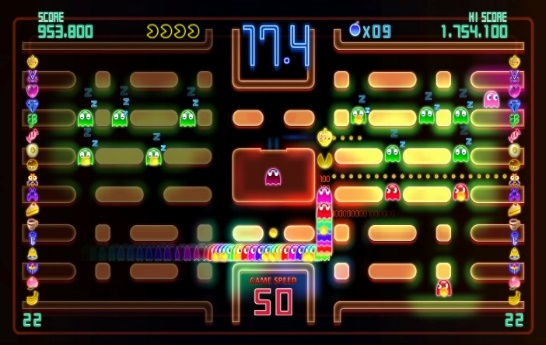
\includegraphics[width=0.50\linewidth]{./img/analysis/champ/midgame.jpg}
\caption{\label{fig:pacman-cs-midgame}Pac-Man CE midgame.}
\end{figure}

Originally released in 2007, Pac-Man CE is of now the last game that series creator Toru Iwatani has worked on.
This game can be considered Iwatani’s faster-paced re-imagining of Pac-Man with modern game design sensibilities.
When distilled, gameplay follows the same timeless loop as the original, but with some new major twists:

\begin{itemize}
\item Pellets only appear in small clusters at defined points in the maze.
Once all the pellets are eaten a bonus fruit appears that will reveal a new cluster.
While I like this change, I believe that this was done to suit the faster-paced gameplay and would be too large of a change for my recreation of the original and may even alienate stakeholders.

\item Sleeping ghosts can found across the maze, who will wake up and pursue Pac-Man when he moves past them.
This is to incentivise the player to get along trial of ghosts behind them, only to get a power pellet and eat them all in a row.
This adds another loop to gameplay alongside eating pellets which is very satisfying to execute properly.
But like the clusters, I believe that this is too much of a far cry from the original game I am trying to replicate.
The long trail of ghosts can clog up the smaller maze of the original and while it should be trivial to instance all those ghosts using OOP, the sheer number can be too much for Python and Pygame.
Performance issues can be encountered that I may not have enough time to solve.
\end{itemize}

\begin{figure}[htbp]
\centering
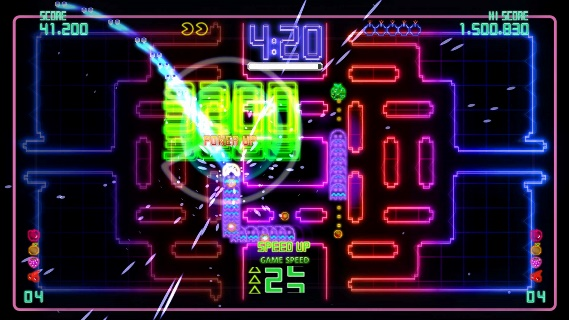
\includegraphics[width=0.50\linewidth]{./img/analysis/champ/eating.jpg}
\caption{\label{fig:pacman-eating}The player eating a trail of ghosts behind them.}
\end{figure}

\begin{itemize}
\item Assistive effects are also added.
Game speed slows down when Pac-Man is close to a pursuing ghost.
Pac-Man can also use bombs to send all the ghosts back into their house at the cost of restarting the dot multiplier.
I understand the need for slow motion since this game is significantly faster-paced, I felt like the tension of a ghost almost catching you from behind, only to narrowly escape them by turning a corner is reduced.
I feel like this and the bombs do not gel well with the slower pace of the original.
Though some of my stakeholders likely the children - may want these assistive effects, so I could add them as an option to enable if I have time.
\end{itemize}

\subsection{Pac-Mania}
\label{sec:org2cd9b7f}
\begin{figure}[htbp]
\centering
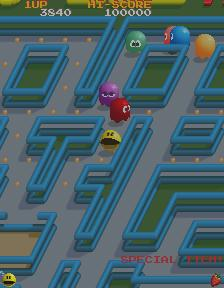
\includegraphics[width=0.33\linewidth]{./img/analysis/mania/midgame.jpg}
\caption{\label{fig:mania-mid}Pac-Mania mid level.}
\end{figure}

Released in 1987 for arcades, Pac-Mania is an isometric representation of the original, with some major additions:

\begin{itemize}
\item Pac-Man can now jump over ghosts to serve as another option to evade them.
This adds a tactical ripple to the gameplay.
This makes more sense in an isometric perspective compared to a top-down one.
While still possible top-down with some dynamic sprite scaling it seems like too much effort to implement into the solution for what it is worth.

\item To balance out the jump, two new ghosts are added.
Funky and Splunky.
Both can jump and Pac-Man cannot jump over Splunky.
Like the jumping mechanic, it seems like this would require a lot of attention to implement properly, which would detract from the quality of the core parts of the solution.
The extra ghosts may also cramp up the small maze and confuse the player.

\item Eating bonus fruit will speed up Pac-Man, serving as a power-up in distancing him from the ghosts, but also a power-down since it makes it harder to navigate the maze.
This seems like a nice twist to gameplay, but I will need to see whether this will play nice in the smaller maze of the original.
\end{itemize}

\subsection{What and What not to Add}
\label{sec:org1d98bae}
Here is a table summarising the extra features that I would like and would not like to feature in my solution.
I feel like my choices show that I only want to make conservative additions/changes.

\begin{center}
\begin{tabularx}{\textwidth}{XXX}
\hline
\textbf{Will Add} & \textbf{Tentative (depends on time left and stakeholder feedback)} & \textbf{Will not Add}\\[0pt]
\hline
Solid colour for maze walls. & Multiple maze layouts (two pairs of tunnels). & Clustered pellets.\\[0pt]
\hline
 & Moving bonus fruit. & Sleeping ghosts.\\[0pt]
\hline
 & Initially random ghost movement. & More than four ghosts.\\[0pt]
\hline
 & Assistive effects like slow-motion and bombs. & Jumping for Pac-Man and ghosts.\\[0pt]
\hline
\end{tabularx}
\end{center}

\subsection{Features of the Solution}
\label{sec:org3a9bac2}
\begin{center}
\begin{tabular}{|l|l|l|l|l|}
\hline
*Feature* & *Source of Feature* & *Essential?* & *Description* & *Explanation* \\
\hline
The player & research & yes & Pac-Man will move & \\
must be able & & & accordingly to the & \\
to control & & & player pressing & \\
Pac-Man in & & & the movement & \\
four & & & keys. & \\
cardinal & & & & \\
directions. & & & & \\
\hline
\end{tabular}
\end{center}

\printbibliography
\end{document}
